\documentclass[10pt]{proc}

\usepackage{cite}
\usepackage[hyphens]{url}  % Allows line breaks at hyphens
\usepackage{hyperref}
\usepackage{dirtytalk}
\usepackage{graphicx}
\usepackage{microtype}

\hypersetup{
    colorlinks=true,
    linkcolor=blue,
    filecolor=blue,      
    urlcolor=blue,
    citecolor=blue,
}


\begin{document}

\title{\textbf{Batch Processing}}
\author{Casper Kristiansson, Nicole Wijkman (Group Therapy)\\[1ex] \today}
\maketitle

\section{Introduction}
In the landscape of data management and processing a solution called batch processing emerged. The solution is powerful and efficient and can process large volumes of data in batches without real-time interactions. The simplification of batch processing is where there is a streamline of tasks that are accumulated over a specific time and then often during periods of low computational demand get executed. Batch processing is the contrast of real-time processing where the requirement for real-time analysis is not needed. In situations where large datasets need to be analyzed and computed there minimal effect to operational delay. While as mentioned it might now offer real-time analysis and automated data handling it still attracts attention from many industries and use cases.

\subsection{Establishing the Cornerstone: The Basics and Fundamentals of Batch Processing}
The core and fundamental principles of batch processing lie within three main principles volume orientation, non-interactivity, and deferred execution \cite{amazonWhatBatch}. 

Volume orientation captures the capability of managing and processing data or transactions in batch processing. Volume orientation uses strategies like concurrent execution and task association to improve the computational efficiency of the different tasks. ‡Non interactivity is one of the key fundamentals where batch processing operates autonomously without the need for real-time user interaction. Lastly, deferred execution involves scheduling jobs during low computational needs of an operation to reduce the computational demand and optimize resource utilization. These three fundamental principles of batch processing allow a robust, efficient, and automated way to manage and compute large volumes of data.

The key components and architecture of batch processing involve \textbf{jobs, batches, job schedulers}, and \textbf{resource management}. A job refers to a single unit of work or a specific task while a batch highlights one or more jobs bundled together which is meant to be processed together to improve computational efficiency. \textbf{Job schedulers} have the task of determining when and in what order different jobs are to be executed. It also has the job of managing dependencies and optimizing workloads. Lastly, \textbf{resource management} has the job allocation and de-allocation of computational resources to ensure that jobs are executed in the best and most efficient way possible.

As already mentioned batch processing has a wide range of application domains where numerous different industries and fields use this type of technology to efficiently improve their operational workflows. For example in the finance sector batch processing is used to manage and execute bulks of transactions, and data analysis to improve the operations of the financial system while ensuring accuracy \cite{advsysconBatchProcessing}. Another example is healthcare where batch processing is used to handle everything from administrational tasks such as billing and insurance claims to data analyses of data to generate insight and update records while ensuring accuracy. 

\subsection{Navigating Through Complexities: Challenges and Solutions in Batch Processing}

Batch processing, despite its advantages, also presents inherent challenges and drawbacks. One prominent challenge is the absence of real-time processing capabilities \cite{memphisdev}. It is often required by organizations for data handling to be instantaneous, in an effort to respond to changing conditions and make timely decisions. Traditional batch processing may fall short of meeting this demand. Cloud-based products have evolved to address this challenge effectively \cite{memphisdev}. These cloud platforms offer features like live stream data processing and dynamic scaling of hardware resources, in turn enabling real-time data analysis and immediate actionable results.

Cloud products also have the potential to significantly enhance scalability and flexibility\cite{memphisdev}. The ability to scale hardware resources up and down as needed allows organizations to adapt to varying workloads and efficiently utilize computing power. This adaptability is similar to batch processing, where tasks can be executed during off-peak times when resources are more readily available.

Batch processing has however also evolved to address some of its inherent challenges. Batch processing solutions have introduced optimizations such as parallelism, load balancing, and data partitioning which enhance both performance and scalability \cite{memphisdev}. Modern batch processing systems also incorporate error handling and retry mechanisms, which ensures both data integrity and reliability \cite{memphisdev}. Thus, in scenarios where real-time processing is not critical, there is a continued relevance of batch processing.  It is also very useful in situations where organizations require efficient processing of extensive data volumes at their convenience.

\section{MapReduce: Simplified Data Processing on Large Clusters}

The Paper "MapReduce: Simplified Data Processing on Large Clusters" by Jeffrey Dean and Sanjay Ghemawat \cite{dean2008mapreduce} came up with a programming model called MapReduce. The paper discusses the challenges in large-scale data processing where it is difficult to manage parallelization, fault tolerance, data distribution, and load balancing. The paper introduces a new programming model that has a straightforward approach to solving these issues which involves mapping data and then reducing it when processing it.

\subsection{Motivation} \label{Motivation1}
In the current technological era, the increase of data collected has increased exponentially where every user interaction and everything that happens around us is collected. The exploration, extraction, and processing of the data require a pipeline that is efficient, scalable, and reliable.

\subsubsection{Scalability Challenges in Data Processing}  \label{ScalabilityChallenge}
The first challenge to data processing is managing and processing data that could be in the sizes of petabytes or even exabytes. This means that there has to be an approach that is able to scale up and is able to process these huge amounts of volumes of data. In order to fulfill this requirement designing algorithms that in an efficient way can process these large-scale data without affecting performance becomes extremely difficult \cite{dhaduk2022challenges}.

While the software approach for dealing with large-scale data processing is one part another issue is the infrastructure limitations. There are a lot of difficult issues and limitations regarding the hardware required to be able to keep up with the volumes of data processed. But with these hardware and infrastructure issues, there are some strategies for optimizing the processing like distributed data processing, parallel processing, and resource utilization. But each of these categories comes with its own set of challenges.

\subsubsection{Complexity of Parallel and Distributed Computing}
When it comes to optimizing the infrastructure and hardware parallel and distributed computing is extremely important. However, designing an algorithm that is suitable for parallel execution is extremely difficult. Some issues for example are synchronization (synchronise tasks to prevent race conditions and deadlocks) and data consistency (ensuring data consistency across multiple nodes).

But building a good system that is in a good way able to distribute tasks in a good way has also other complexities such as data partitioning (evenly distributing data across nodes), task scheduling (scheduling tasks to maximize resource utilization), resource management (optimizing the allocation of resources), error handling and recover (identify errors regarding distributing tasks and able to recover corrupted data) \cite{singh2013review}.

\subsubsection{Reliability and Fault Tolerance} \label{Reliability}
Another extremely important point is ensuring reliability and fault tolerance when processing data. When processing data failure is something that is normal and not an exception. This means that in large-scale system failures among clusters, hardware or software is common. However, building a workflow that is able to synchronize data when failure happens becomes extremely complicated and complex. This means that reaching a totally robust system that is able to handle fault tolerance becomes hard \cite{singh2013review}.

\subsection{Contributions and Solutions}
With all of these existing issues and challenges, Jeffrey Dean and Sanjay Ghemawat who presented the paper on MapReduce want to confront and solve the challenges. The paper introduces a programming model that revolutionizes the approach to large-scale data processing by solving some of the problems mentioned in \ref{Motivation1}.

\subsubsection{Simplified Programming Model for Large-Scale Data Processing} \label{constribution1}
One of the main reasons why MapReduce was groundbreaking was due to the simplification of usage among developers \cite{dean2008mapreduce}. A developer that wanted to utilize MapReduce generally speaking only required to specify two functions \textbf{Map} and \textbf{Reduce}. The function Map processes input data a produces intermediate key value pairs. The function Reduce then takes these key-value pairs and aggregates them to produce the final result. As seen in figure \ref{fig:enter-label} MapReduce does have a shuffling phase which has the purpose of rearranging intermediate key-value pairs to ensure that associated keys are processed by the same reducer.

\begin{figure}[!h]
    \centering
    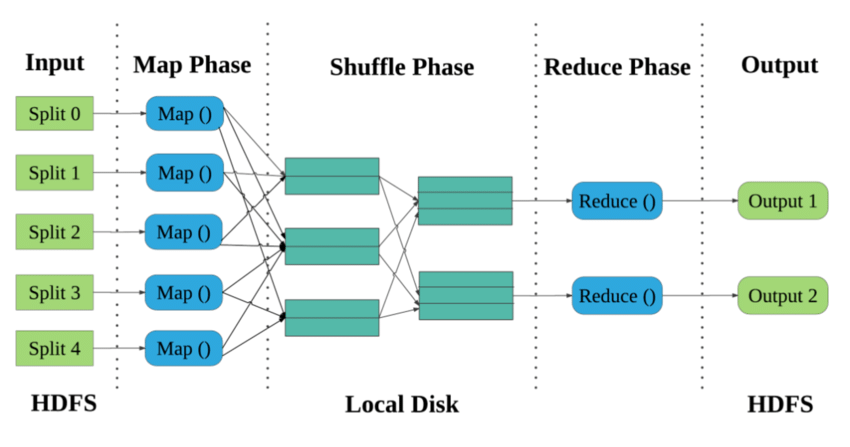
\includegraphics[width=1\linewidth]{The-Structure-of-MapReduce-Model.png}
    \caption{The Basic Structure of Map Reduce \cite{mapreduceModel2023}}
    \label{fig:enter-label}
\end{figure}

With this kind of system developers only needed to think about computation and not system details. This means that the abstract model handles tasks such as partitioning scheduling, inter-node communication, and fault tolerance.

Having this type of model allows a developer to solely focus on writing the actual data processing logic which allows a better workflow of configuring and creating data processing systems. Having this simple structure allows for an easy learning curve by allowing developers to use it without expertise in parallel and distributed systems.

MapReduce also became extremely popular due to the programming model being applicable to a wide variety of problem types including the different types and formats of data. For example, developers can process unstructured data or structured data. 

\subsubsection{Automatic Management of Parallelization, Data Distribution, and Fault Tolerance}
As mentioned in \ref{constribution1} MapReduce allows developers to not focus on what happens under the hood. MapReduce dynamically assigns tasks which means that it automatically divides input data into chunks and assigns them to a batch (Map Task) which then is executed in parallel. The  \textbf{Map} function creates intermediate key-value pairs that tasks are then partitioned into regions which then are managed by different Reduce tasks. With the help of load balancing this allows for balanced workloads where the system resources are balanced across all worker nodes.

While MapReduce manages these types of actions the system also has optimized internal operations. For example, a big thing about MapReduce is the data placement (for example within a distributed file system), so that data is not required to move a lot which minimizes data movement across networks. The data is also processed locally where the input data is stored or nearby to reduce the network usage.

Furthermore, the system allows for automated fault tolerance and recovery. If faults happen with tasks the system will automatically re-execute failed tasks ensuring that the task gets executed. Any intermediate data is stored on disk which means that if any node failures or task failures would have happen the data could still be recovered.

\subsubsection{Scalability and Applicability Across Varied Real-World Use Cases}
With the help of all of these different processes, the scalability with the help of MapReduce is really good. It has a proven ability to be able to process petabytes of data while efficiently scaling and adding computing nodes to make use of the available system resources.

MapReduce has been applicable to a wide range of different applications like web search, graph processing, and distributed sorting. The programming model has proven to be effective across different computing environments and utilizing computer resources in a cluster effectively. It has also shown it is able to in a robust way deal with task and node failures while ensuring stability and reliability.

\subsection{Your Opinion}
MapReduce which was introduced by Jeffrey Dean and Sanjay Ghemawat has proven to be useful. They came up with a programming model that had a straightforward approach to managing massive amounts of data by solving it using a steps system; Map, and Reduce.

\subsubsection{The Elegant Solution of Simplification and Abstraction}
The proposed programming model provides an elegant and simple solution with the Map and Reduce functions. Keeping it to this level of simplification allows developers to effortlessly parallelize computations without having a steep learning curve. However, keeping it simplified limits the flexibility of usage for certain algorithms and computations that don't fit well with the MapReduce model.

As mentioned in \ref{constribution1} MapReduce provides an abstraction to avoid complexity in what happens behind the scenes for example handling parallelization, distributions of data, and fault tolerance. But because of this, it does introduce ineffective specific tasks that might be improved with the help of fine-graining the data flow and task execution.

\subsubsection{Remarkable Scalability and Fault Tolerance}
MapReduce has proven to be able to scale across nodes and processes to massively increase data processing while still being able to handle fault tolerance. It has built-in workflows for handling node failures, task executions, and data recovery. The approach that the authors of the paper on MapReduce took to manage and utilize system resources might not be optimal in all situations. For example, it has been proven to be inefficient when variable tasks demand. MapReduce uses a predefined scheduling which means that it is not able to adapt well in a dynamic environment where resource changes happen during runtime.


\section{Resilient Distributed Data-sets: A Fault-Tolerant Abstraction for In-Memory Cluster Computing}

The paper 'Resilient Distributed Datasets: A Fault-Tolerant Abstraction for In-Memory Cluster Computing' by Matei Zaharia et al. \cite{RDDs} presents a solution to the challenges in large-scale data processing and distributed computing. It addresses the inefficiencies in existing frameworks when reusing data across multiple computations, especially in iterative algorithms and interactive data mining scenarios. The paper introduces Resilient Distributed Datasets (RDDs), a game-changing data-sharing abstraction for in-memory cluster computing.

\subsection{Motivation}
%Describe the motivation of the papers in your selected module. \textbf{WHY} is the addressed problem interesting and important to be solved?

The motivation behind the paper \say{Resilient Distributed Datasets: A Fault-Tolerant Abstraction for In-Memory Cluster Computing} is rooted in addressing some critical challenges of large-scale data processing and distributed computing. 

\subsubsection{Inefficiencies with Existing Frameworks}
One of the central motivations of this paper is the inefficiencies that are inherent in existing distributed computing frameworks. These inefficiencies become especially clear when reusing data across multiple computations, and they can have a large impact on the overall performance of data-intensive applications. This paper thus emphasizes the performance gains achievable through in-memory data retention.

\subsubsection{Fault Tolerance}
Another key motivation that is highlighted throughout the paper is the need for robust fault tolerance mechanisms and a versatile programming model. As can be seen in Section \ref{Reliability}, ensuring system reliability is crucial as large-scale clusters become more complex and the volume of data being processed continues to grow.

\subsubsection{Streamlining Data Processing}
To summarise, the primary goal of the paper is to streamline data processing in large-scale scale cluster computing environments. The authors aim to do this by addressing the inefficiencies in existing frameworks, enhancing fault tolerance, and providing a versatile programming model. This motivation aligns with the growing need for scalable and reliable data processing solutions, discussed in Section \ref{ScalabilityChallenge}.

\subsection{Contributions and Solutions}
%Explain the main contributions of the papers. \textbf{WHAT} are the solved problems?
%You may optionally use a list of contributions. For example:
%\begin{itemize}
% \item First contribution
% \item Second contribution
% \item Third contribution
%\end{itemize}

The paper presents significant contributions to the field of distributed computing, enabling more efficient and versatile data processing. The authors' solution revolves around the introduction and effective use of RDDs to provide fault-tolerant, in-memory data sharing, and versatile support for different programming models in distributed cluster computing. RDDs offer a promising approach to solving the addressed problems in a more efficient and expressive manner.

\subsubsection{Introduction of RDDs} 
The primary contribution of the paper is the introduction of RDDs as an efficient data-sharing abstraction for large-scale cluster computing. RDDs serve as a fundamental building block for in-memory cluster computing, addressing the challenge of reusing data across multiple computations.

RDDs are introduced as an efficient and fault-tolerant data abstraction. They are created through coarse-grained transformations (e.g., map, filter, join) on distributed datasets, offering lineage information for efficient data recovery in case of node failures.
    
\subsubsection{Improved Fault-Tolerance}
RDDs offer a fault-tolerant mechanism for distributed computing. This is done through a lineage-based recovery approach, which ensures that lost data partitions can be efficiently recomputed without the need for costly data replication or extensive disk I/O. This contributes to the robustness and reliability of distributed applications.

RDDs use lineage information to recover lost data partitions, rather than relying on data replication. By tracking the sequence of transformations applied to the data, RDDs can recompute lost partitions, minimizing the impact of failures on application performance.
    
\subsubsection{Diverse Programming Model Support}
RDDs are shown to be versatile and expressive, capable of accommodating various parallel programming models, including MapReduce, Dryad, Pregel, and more. This flexibility enables RDDs to address problems that were not adequately covered by existing specialized models, as well as to support a broad spectrum of applications, from iterative algorithms to interactive data mining.

RDDs provide a versatile programming model that allows users to express a wide range of parallel applications. They can replace or complement specialized models like MapReduce, Dryad, and Pregel, enhancing flexibility in addressing various computation needs.

\subsection{Your Opinion}
%What do you think about these papers? List their strong and weak points. Is the solution good? How good is the evaluation of the work? What are the disadvantages and shortcomings of the solution given by the authors? Did the authors overlook anything during the evaluation of their solution?

The paper \say{Resilient Distributed Datasets: A Fault-Tolerant Abstraction for In-Memory Cluster Computing} introduces concepts and solutions to the field of distributed computing. In this section, I will discuss the strong and weak points of the paper and evaluate the authors' work.

\subsubsection{Strengths}
I believe that the introduction of RDDs as an efficient data-sharing abstraction is a very significant contribution. It addresses the challenge of reusing data across multiple computations as well as promoting more efficient and faster data processing.

Another strong point is the paper's emphasis on supporting diverse programming models through RDDs. RDDs can accommodate various parallel programming paradigms, making them adaptable to a wide range of applications. This enhances the flexibility of distributed computing. I also believe that the authors' decision to open-source the Spark system, which implements RDDs, is a positive step toward fostering collaboration and innovation in scalable data analysis and systems research.

\subsubsection{Weaknesses}

While RDDs simplify many aspects of distributed computing, as with any new technology they might introduce a learning curve for users accustomed to other approaches. It is also worth noting that while RDDs offer substantial performance improvements, one must recognize that there may still be limitations in handling certain types of computations or algorithms efficiently. I also think the paper could expand by further discussing scenarios where RDDs may not be the ideal choice. RDDs seem well-suited for static environments, but I would have liked to see their adaptability to dynamic environments with varying resource demands be explored further. Something I was curious about is how RDDs perform when resource changes occur during runtime.

\subsubsection{Conclusion}

In conclusion, I believe that the paper introduces valuable concepts and solutions with RDDs, significantly improving the efficiency and versatility of distributed computing. I believe that the paper's evaluation of the work is very strong, as there are comprehensive performance checks and explanations to provide a more nuanced understanding of RDDs' advantages and limitations. While there are some areas that could be further explored and refined, RDDs definitely offer a promising approach to solving key challenges in the field.

\bibliographystyle{IEEEtran}
\bibliography{main}

\end{document}
